\documentclass[12pt,a4paper]{article}
\usepackage{fancyvrb}
\usepackage{fancypar}
\usepackage[center]{qtree}
\usepackage{listings}
\usepackage{graphicx}
\usepackage{hyperref}

\author{John S. Fourkiotis}
\title{cmake 101}
\begin{document}
\maketitle
\tableofcontents
\section*{License}
This article is Copyright (C) 2011 by Ioannis S. Fourkiotis. You are free to distribute this article to anyone you want, so long as you do not charge anything for it, and it is not altered. You must give away the article in its entirety, or not at all.
\section{Introduction}
This article presents a simple introduction to the \verb+cmake+\footnote{see \href{www.cmake.org}{www.cmake.org}} build system. The \emph{audience} of this article should be engineers and scientists that use \verb|C/C++| in their applications and research. This article is not a full-blown tutorial of \verb+cmake+. It just presents the amount of information needed to develop a simple \emph{application} or \emph{project}. This information is presented through building a simple math library that is used from other simple programs. All sources used in this article are hosted in \verb|git| \footnote{check \href{www.github.com}{www.github.com}}. To grab them, just use \verb|git clone git://github.com/jstark/cmake101| \footnote{grab git from \href{http://git-scm.com/download}{http://git-scm.com/download}}. The tutorial assumes a UNIX or GNU/Linux OS, with \verb+cmake+ installed. If you run a Windows box, check the appendix for instructions.
\section{The quadratic equation}
The first program that I write to learn a new programming language is one that finds the roots of the world-famous (I hope) \emph{quadratic equation}. The quadratic equation is given by:
\begin{equation}
ax^2+bx+c = 0
\end{equation}
where coefficients $a,b,c\in \Re$ and $a\neq0$. The coefficients $a,b$ and $c$ could also be \emph{complex} numbers, but let's keep things simple. 

Whether a quadratic equation has complex or real roots depends on the value of the \emph{discriminant} $\delta$ which is equal to:
\[
\delta = b^2-4ac
\]

The discriminant can be $0$, negative or positive. If it is positive, then equation (1) has two dinstict real roots, $x_1$ and $x_2$ given by:
\[
x_{1,2} = \frac{-b\pm\sqrt{\delta}}{2a}
\]

If the discriminant is $0$, then there are two identical real roots, e.g $x_1=x_2$ given by:
\[
x_1=x_2=\frac{-b}{2a}
\]

If the discriminant is negative, then the quadratic equation has two complex roots. The two complex roots are given by:
\[
x_{1,2}=\frac{-b\pm i\sqrt{\delta}}{2a}
\]
where $i$ is the square root of $-1$. For those interested in the details, check the wiki article \href{http://en.wikipedia.org/wiki/Quadratic\_equation}{http://en.wikipedia.org/wiki/Quadratic\_equation}.

\section{Starting up the project}
Let's say that we want to build a simple application that will ask the user to type the three coefficients, and then present the roots of the quadratic equation. Because our quadratic equation solver will be used by many programs, we want it to be in a library (\emph{shared} or \emph{static}) that will be used from our programs. We also want to include some tests for our library, so that we can be sure that any changes we make to the code, won't create any bugs in our solver. 

Our quadratic equation solver won't be our only math functionality offered by our library. It will be just the first. We can think of it as the first component of a library. Let's name this library as \verb+eqsolver+, which will also be our project name. To start up our project, we can take the following easy steps:

\begin{description}
\item [Create a project skeleton] For our little project, we need to create a root directory named \verb+eqsolve+ and add to it two more directories, \verb+src+, which will hold our source files, and \verb+test+
which will hold simple library tests.
\item [Add \texttt{cmake} support] To make the project \emph{understandable} for \verb+cmake+, add a file named \verb+CMakeLists.txt+ \emph{to each of our directories}. We will add to these files later.
\item [Add the source files] Add a header file named \verb+eqsolver.h+ and a source file named \verb+quad.cpp+ to the source folder \verb+src+. We will add code to these files in the following section. 
\end{description}

Our project structure should now look more or less this:

\begin{table}[htdp]
%\caption{Project directory structure}
\begin{center}
\begin{tabular}[c]{@{}l@{}}
\Tree [.\framebox[2cm]{eqsolver} [.CMakeLists.txt ] [.\framebox[2cm]{src} CMakeLists.txt ] [.\framebox[2cm]{test} CMakeLists.txt eqsolver.h quad.cpp ] ]
\end{tabular}
\end{center}
\end{table}

We will add files to the \verb+src+ directory later. 

\section{\texttt{cmake} setup}
Now that our project structure is ready, we can add some \verb+cmake+ \emph{scripting code} to the three \verb+CMakeLists.txt+ files. Add the following lines to the first file, in \verb+eqsolver+ directory:

\begin{Verbatim}[numbers=left, frame=lines, label=file \texttt{eqsolver/CMakeLists.txt}]
cmake_minimum_required (VERSION 2.6)

project (eqsolver)

add_subdirectory (src)

enable_testing()
add_subdirectory (test)
\end{Verbatim}

At the first line, we require a \verb+cmake+ version of at least 2.6. Then we name our project (at line 3), and state that there are two more directories (\verb+src+ and \verb+test+) in this project, that need processing by \verb+cmake+. We state this by using the \verb+add_subdirectory+ command. Each directory that is added by using \verb+add_subdirectory+ must contain another \verb+CMakeLists.txt+ file, that describes to \verb+cmake+ what to do in that directory. 

The \verb+CMakeLists.txt+ file inside \verb+src+ directory contains the following commands:

\begin{Verbatim}[numbers=left, frame=lines, label=file \texttt{eqsolver/src/CMakeLists.txt}]
include_directories(.)

SET(source_code eqsolver.h quad.cpp)

add_library (eqsolver SHARED ${source_code})

install (TARGETS eqsolver DESTINATION "${PROJECT_BINARY_DIR}/lib")
install (FILES eqsolver.h DESTINATION "${PROJECT_BINARY_DIR}/include")
\end{Verbatim}

At the first line, we state that this directory should be searchable for include files, during the project compilation. Then, we create a \emph{set} that we name as \verb+source_code+. This set contains our source files. At line 5, we state that there is a \emph{target} in this directory, which is named \verb+eqsolver+. This target is a \emph{shared} library (\verb+dll+ for windows, \verb+dylib+ for Mac OS X, and a \verb+so+ for unix/linux), and depends on the files contained in the \verb+source_code+. In other words, we ask \verb+cmake+, to build a shared library based on \verb+eqsolver.h+ and \verb+quad.cpp+. After the build process is completed, we state that the library executable should be copied to a directory named \verb+lib+ and that the header \verb+eqsolver.h+ should be copied to a directory named \verb+include+. These directories will be created in the folder that is the \emph{build} folder. A \emph{build} folder can be any directory. The \verb+PROJECT_BINARY_DIR+ denotes the build folder. We leave empty our last \verb+CMakeLists.txt+ for now. 

The \verb+eqsolver.h+ file contains the declaration of our function, \verb+solve_quadratic_eq+ plus one other stuff that should be familiar to you, regarding header guards, symbol exporting from libraries (\verb+DLL_PUBLIC+) and compilation and linking to \verb|C/C++| applications.

\lstset{language=C++}
\begin{lstlisting}[basicstyle=\small, numbers=left,caption=eqsolver.h,columns=flexible,keywordstyle=\color{black}\ttfamily]
#ifndef eqsolver_h
#define eqsolver_h

#if defined _WIN32 || defined __CYGWIN__
	#ifdef eqsolver_EXPORTS // define this when generating DLL
		#ifdef __GNUC__
			#define DLL_PUBLIC __attribute__((dllexport))
		#else
			#define DLL_PUBLIC __declspec(dllexport)
		#endif 
	#else
		#ifdef __GNUC__
			#define DLL_PUBLIC __attribute__((dllimport))
		#else
			#define DLL_PUBLIC __declspec(dllimport)
		#endif
	#endif
	#define DLL_HIDDEN 
#else
	#if __GNUC__ >= 4
		#define DLL_PUBLIC __attribute__ ((visibility("default"))) 
		#define DLL_HIDDEN __attribute__ ((visibility("hidden")))
	#else
		#define DLL_PUBLIC 
		#define DLL_HIDDEN
	#endif
#endif

#ifdef __cplusplus
extern "C" {
#endif

DLL_PUBLIC int solve_quadratic_eq(const double (*coeffs)[3], double (*roots)[4]);

#ifdef __cplusplus
}
#endif

#endif /* eqsolver.h */
\end{lstlisting}

The file \verb+quad.cpp+\footnote{The currently implemented solution suffers from numerical problems. Check the wikipedia article for more information} contains a simple implementation of our library's function, plus some helper
functions that we won't export to the user:
\begin{lstlisting}[basicstyle=\small, numbers=left,caption=quad.cpp,columns=flexible,keywordstyle=\color{black}\ttfamily]
#include "eqsolver.h"
#include <cmath>

const double zero_tol = 1.0e-06;

static double discriminant(const double (*coeffs)[3])
{
	return (*coeffs)[1] * (*coeffs)[1] - 4.0 * (*coeffs)[0] * (*coeffs)[2];
}

int solve_quadratic_eq(const double (*coeffs)[3], double (*roots)[4])
{
	// find discriminant and then calculate roots
	double d = discriminant(coeffs);
	
	int retCode = 0;
	if (d > zero_tol) // two real roots
	{
		double d1 = (-(*coeffs)[1]+sqrt(d))/(2.0* (*coeffs)[0]);
		double d2 = (-(*coeffs)[1]-sqrt(d))/(2.0* (*coeffs)[0]);
		(*roots)[0] = d1;
		(*roots)[1] = d2;
	} else if (d < -zero_tol) // complex roots
	{
		double r = (-(*coeffs)[1])/(2.0*(*coeffs)[0]);
		double w = (sqrt(d)/(2.0*(*coeffs)[0]));
		(*roots)[0] = r; // first root is x1 = r + iw,
		(*roots)[1] = w; // real part is roots[0], imaginary is roots[1]]
		(*roots)[2] = r; // second root is x2 = r - iw,
		(*roots)[3] = -w; //real part is roots[2], imaginary is roots[2]
		retCode = 1;
	} else // two identical real roots
	{
		double r = (-(*coeffs)[1])/(2.0*(*coeffs)[0]);
		(*roots)[0] = r;
		(*roots)[1] = r;
	} 
	return retCode;
}
\end{lstlisting}
\section{Building our project}
Now we can try building our project. To do that, create a new directory, named \verb+build+ inside the main directory \verb+eqsolver+. Change to the build directory, and type \verb+cmake ../+ to build the project. \verb+cmake+ will run a bunch of tests to check what compilers are available. If no error was encountered, you will notice that lots of files and directories have been created inside the build directory. If you are on a GNU/Linux or UNIX box, you will also notice a \verb+Makefile+. Type \verb+make+ to build the project. If no errors were encountered (check your source files if errors were encountered), you will notified that the project was built. In my computer, the output from the \verb+make+ command is looks like the following:

\begin{Verbatim}
Scanning dependencies of target eqsolver
[100%] Building CXX object src/CMakeFiles/eqsolver.dir/quad.cpp.o
Linking CXX shared library libeqsolver.dylib
[100%] Built target eqsolver
\end{Verbatim}

After our project is build, we can \emph{install} it. Type \verb+make install+. You will notice that two folders were created inside the \emph{build} directory, one named \emph{include}, and one named \emph{lib}. Check the contents of these directories. They should contain the headed \verb+eqsolver.h+ and the our dynamic library. You can now give these two folders with their contents to someone else to use your library. 

\section{Adding tests}
To be sure that our library works as expected, we should create a couple of tests to test the functionality. First of all, we must check that our library can be used from \verb+C+ and \verb|C++| code. Create two directories inside the \verb+test+ directory, named \verb+test_link_cpp+ and \verb+test_link_c+. Add a \verb+CMakeLists.txt+ file in each one. Add a source file named \verb+main.cpp+ in \verb+test_link_cpp+ and a source file named \verb+main.c+ in \verb+test_link_c+. The \verb+test+ directory should look like this:

\begin{table}[htdp]
%\caption{Project directory structure}
\begin{center}
\begin{tabular}[c]{@{}l@{}}
\Tree [.\framebox[2cm]{test} [.CMakeLists.txt ] [.\framebox[2cm]{test\_link\_cpp} CMakeLists.txt main.cpp ] [.\framebox[2cm]{test\_link\_c} CMakeLists.txt main.c ] ]
\end{tabular}
\end{center}
\end{table}

Let's add the necessary commands to our new \verb+CMakeLists.txt+ files. In the \verb+CMakeLists.txt+ inside the \verb+test+ directory, add the following commands:

\begin{Verbatim}[numbers=left, frame=lines, label=file \texttt{eqsolver/test/CMakeLists.txt}]
include_directories(../src)

add_subdirectory (test_link_cpp) 
add_subdirectory (test_link_c)

add_test (test1 ${CMAKE_BINARY_DIR}/test/test_link_cpp/test1)
add_test (test2 ${CMAKE_BINARY_DIR}/test/test_link_c/test2)
# we can add more tests here

\end{Verbatim}

The first three commands should be familiar to you. We are stating that during all test compilation, the compiler should also check our \verb+src+ directory for include files. Then, we add our test directories (lines 3 and 4). The interesting lines are 6 and 7, where we \emph{create} two tests, one named \verb+test1+ and one named \verb+test2+. The first test, \verb+test1+, will run the executable named \verb+test1+ inside the \verb+test/test_link_cpp+ directory, and the second test, \verb+test2+, will run the executable \verb+test2+ inside the \verb+test/test_link_c+ directory.

Edit the \verb+CMakeLists.txt+ inside the \verb+test_link_cpp+ directory, and add the following commands:
\begin{Verbatim}[numbers=left, frame=lines, label=file \texttt{eqsolver/test/test\_link\_cpp/CMakeLists.txt}]
set (source_code main.cpp)

add_executable (test1 {source_code})

target_link_libraries (test1 eqsolver)

\end{Verbatim}

At line 3, we ask the build system to create an executable named \verb+test1+ that depends on \verb+main.cpp+.
The other interesting command here, is the one at line 5, where we ask the build system to link with our library. 

Our last \verb+CMakeLists.txt+ is very similar:
\begin{Verbatim}[numbers=left, frame=lines, label=file \texttt{eqsolver/test/test\_link\_c/CMakeLists.txt}]
set (source_code main.c)

add_executable (test2 ${source_code})

target_link_libraries (test2 eqsolver)

\end{Verbatim}

Now we must add some code to our test source files, \verb+main.cpp+ and \verb+main.c+. Add the following code to \verb+main.cpp+:
\begin{lstlisting}[basicstyle=\small, numbers=left,caption=main.cpp,columns=flexible,keywordstyle=\color{black}\ttfamily]
#include <stdio.h>
#include "eqsolver.h"

int main(int argc, char *argv[])
{
        typedef int (*solve_fun)(const double (*c)[3], double (*r)[4]);

        solve_fun sf = solve_quadratic_eq;
        return 0;
}  
\end{lstlisting}

Add the very same code to \verb+main.c+. Now we are ready to test if our two tests can link with our library. To check this, change to the \emph{build} directory, and rerun the \verb+cmake ../+ command. Then build the library by typing \verb+make+. To run the tests, type \verb+make test+. You should see something like the following output:

\begin{Verbatim}
Running tests...
Test project ../eqsolver/build
    Start 1: test1
1/2 Test #1: test1 ............................   Passed    0.00 sec
    Start 2: test2
2/2 Test #2: test2 ............................   Passed    0.00 sec

100% tests passed, 0 tests failed out of 2

Total Test time (real) =   3.01 sec
\end{Verbatim}

\section{Adding more tests}
To actually test whether our library works correctly, we can create a \emph{unit} test. In this test, we must check if the function \verb+solve_quadratic_eq+ produces the right results for various inputs. The following table contains some possible values for the coefficients $a,b$ and $c$, and the respective solutions:

\begin{table}[htdp]
\caption{test values}
\begin{center}
\begin{tabular}{|c|c|c|c|c|}
\hline
a & b & c & $x_{1}$ & $x_{2}$ \\
\hline
$1$ & $2$ & $3$ & $-1+1.4142i$ & $-1-1.4142i$ \\
$1$ & $-2$ & $-3$ & $3$ & $-1$ \\
$1$ & $-5$ & $1$ & $4.7913$ & $0.20871$ \\
$1$ & $-2$ & $1$ & $1$ & $1$\\
\hline 
\end{tabular}
\end{center}
\label{default}
\end{table}%
Create a new directory named \verb+unit_test_1+ inside our \verb+test+ directory. Add this new directory
to the build system, by adding the following commands (shown in red) to \verb+test/CMakeLists.txt+:
\begin{Verbatim}[commandchars=\\\{\}, numbers=left, frame=lines, label=file \texttt{eqsolver/test/CMakeLists.txt}]
include_directories(../src)

add_subdirectory (test_link_cpp) 
add_subdirectory (test_link_c)
\textcolor{red}{add_subdirectory} (unit_test_1)

add_test (test1 ${CMAKE_BINARY_DIR}/test/test_link_cpp/test1)
add_test (test2 ${CMAKE_BINARY_DIR}/test/test_link_c/test2)
\textcolor{red}{add_test} (test3 ${CMAKE_BINARY_DIR}/test/unit_test_1/test3)
\textcolor{red}{set_tests_properties} (test3 PROPERTIES PASS_REGULAR_EXPRESSION  
"ret 1, roots -1.000000 1.414200 -1.000000 -1.414200
ret 0, roots 3.000000 -1.000000 0.000000 0.000000
ret 0, roots 4.791300 0.208710 0.000000 0.000000
ret 0, roots 1.000000 1.000000 0.000000 0.000000")

\end{Verbatim}
For the third test, we add a \emph{property} that states that the output of the test should match the string:
\begin{Verbatim}
"ret 1, roots -1.000000 1.414200 -1.000000 -1.414200
ret 0, roots 3.000000 -1.000000 0.000000 0.000000
ret 0, roots 4.791300 0.208710 0.000000 0.000000
ret 0, roots 1.000000 1.000000 0.000000 0.000000"
\end{Verbatim}

Now, create a new \verb+CMakeLists.txt+ inside the \verb+unit_test_1+, and add the following commands:
\begin{Verbatim}[numbers=left, frame=lines, label=file \texttt{eqsolver/test/unit\_test\_1/CMakeLists.txt}]
set (source_code main.cpp)

add_executable (test3 ${source_code})

target_link_libraries (test3 eqsolver)
\end{Verbatim}

The \verb+main.cpp+ should test the function \verb+solve_quadratic_eq+ on the values of table 1. The following listing shows the code:
\begin{lstlisting}[basicstyle=\small, numbers=left,caption=main.cpp,columns=flexible,keywordstyle=\color{black}\ttfamily]
#include <stdio.h>
#include "eqsolver.h"

int main(int argc, char *argv[])
{
	const int CASES = 4;
	const double COEFFS[CASES][7] = {
			{1, 2, 3, -1, 1.4142, -1, -1.4142},
			{1,-2,-3,  3, -1, 0, 0},
			{1,-5, 1, 4.7913, 0.20871, 0, 0},
			{1,-2, 1, 1, 1, 0, 0}};

	for (int i = 0; i < CASES; ++i)
	{
			int ret = 0;
			const double C[3] = {COEFFS[i][0], COEFFS[i][1], COEFFS[i][2]};
			double roots[4] = {0};
			ret = solve_quadratic_eq(&C, &roots);
			printf("ret %d, roots %f %f %f %f\n", ret, 
				COEFFS[i][3], COEFFS[i][4], COEFFS[i][5], COEFFS[i][6]);
	}
	return 0;
}
\end{lstlisting}

Now run rebuild the project by typing \verb+cmake ../+ inside the build directory, build the project by typing \verb+make+, and finally rerun the tests, by typing \verb+make test+. You should see no errors.
\section{Exercises}
To further hone your skills, try completing the following exercises:
\begin{enumerate}
\item Add the necessary code to test whether coefficient $a=0$. In this case, make the function \verb+solve_quadratic_eq+ return $-1$. Rebuild the project, and make sure that all tests pass.
\item Expose the function \verb+discriminant+ to the library's users (add it to \verb+eqsolver.h+).
\item Create another unit test for the function \verb+discriminant+. 
\item Build and test the project under other OSes. 
\end{enumerate}

\section{\texttt{cmake} for Windows}
To use \verb+cmake+ under Windows, you should download the software bundle from \href{http://cmake.org/cmake/resources/software.html}{http://cmake.org/cmake/resources/software.html}. Under windows, you should use the \verb+GUI+ version of \verb+cmake+. The main window of that version is shown on the following picture:

\begin{figure}[t]
\centering
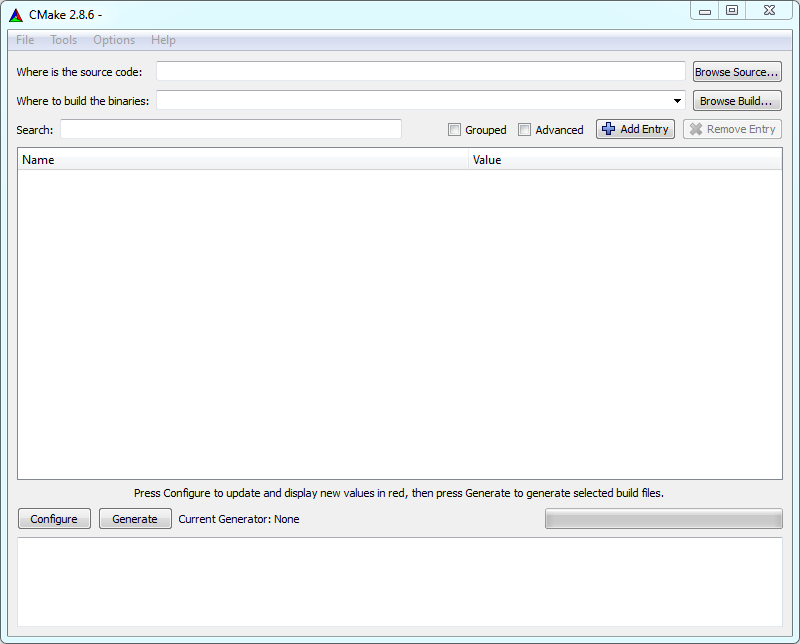
\includegraphics[width=\linewidth]{cmake_gui.png}
\caption{cmake gui}
\end{figure}

There are some easy steps you must take to build the project. First, add the path to the source project directory in the first line edit, with the label ``Where is the source code:''. Then create a \emph{build} directory and add its path to the second line edit labeled ``Where to build the binaries:''. Then press the button labeled ``Configure'' to have \verb+cmake+ test your environment (mainly your compiler tooling). After \verb+cmake+ finished, press the button labeled ``Generate'', to have \verb+cmake+ generate a Visual Studio project. You can then open the project solution with Visual Studio. 

\section{Article revision history}
The following table describes the changes to this article.
\begin{table}[htdp]
\caption{revision history}
\begin{center}
\begin{tabular}{|c|c|}
\hline
Date & Notes \\
\hline
7-Nov-2011 & version 1.0\\
\hline
\end{tabular}
\end{center}
\label{default}
\end{table}%

\end{document}
